\section{模型的建立与求解}

\subsection{相似性度量模型}

\subsubsection{度量角度的确立}

在对小学数学应用题的相似性度量过程中,通常会使用两个依据:

\begin{enumerate}
    \item 根据题干文字进行相似性比对,确定两道题目间题面的相似程度。
    \item 通过人工或机器学习的方式为题目根据知识点进行“标签化”,两道题目之间的标签重合越多,则越相似。
\end{enumerate}

实际上,进行“标签化”对题目进行相似性度量是较为科学且准确的,符合师生快速锁定同类题型进行巩固训练的实际需求,而光凭文本信息进行相似性度量的结果并不符合实际的教育需求。

但仅根据少量题目样本无法将“标签化”过程有效自动化,难以避免通过人工手段为题目加上知识点标签。考虑到平台运营的切实情况,人工进行“标签化”操作成本过大,且判断过程中人为主观因素较多,可能也会导致度量结果出现较大偏差。

因而,本文经过综合考虑,还是选择通过题干文字进行相似性比对进行相似性度量。

\subsubsection{度量过程的关键步骤}


本文将度量过程总结成四个关键步骤以便于读者理解,下文也将围绕这四个关键步骤进行展开:

\begin{enumerate}
    \item 文本预处理
    
    文本预处理是自然语言处理中的重要步骤之一,其目的是将原始的文本数据转换成计算机可以处理的形式。为了提高文本处理任务的效率和准确性,文本预处理是在进行后续分析处理的必要前置步骤。

    \item 借助LDA模型建立相似性矩阵
    \item 使用余弦相似度计算相似性结果
\end{enumerate}

\subsubsection{文本预处理}

首先需要对题目文本进行分词处理,以好通过词袋模型的方式将题目文本进行向量化,进行进一步的研究。因本文研究的题目大多处于中文语言环境下,需先对题目进行分词处理。本文为了研究方便,使用的是被广泛使用的开源中文分词工具jieba。另外也可以使用NLPIR分词系统达到相同效果。NLPIR分词系统是由中国科学技术大学自然语言处理与社会人文计算实验室开发的一款中文自然语言处理工具。它是基于统计和规则两种方法相结合的分词系统,能够对中文文本进行精准的分词和词性标注,完美契合本文的研究需要。

在分词处理的过程中,还需要分离并忽略标点符号、数字、停用词等词语的影响。详细的处理操作可以参考周萍老师在《语义分析及相似性度量方法》\cite{ZhouJiYuYuYiFenXiDeWenBenXiangSiXingDuLiangYanJiuJiYingYong2017}研究中总结的预处理流程。但本文简化了处理流程,仅对分词结果进行了简单的标点符号排除与数字排除,以加快研究进程。

\begin{figure}[htbp]
    \centering
    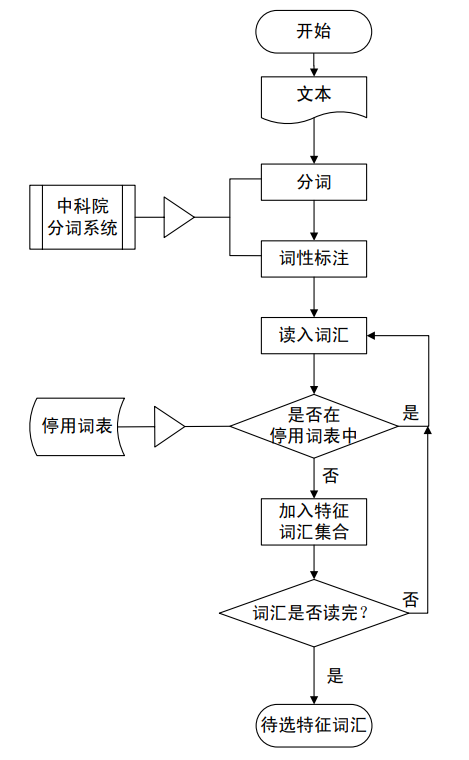
\includegraphics[width=6cm,height=10cm]{res/Text preprocessing process.png}
    \caption{文本预处理流程图}
\end{figure} 

在这里也给出一段进行文字预处理的Python代码以作参考,并作为后续研究的前提:

\begin{mgCodeBlock}[Python 文字预处理代码]
    \VerbatimInput{res/participle.py}
\end{mgCodeBlock}

\subsubsection{借助LDA模型建立相似性矩阵}

若仅通过传统方式进行普通的“文字对比”,可以采取TF-IDF分析文本中的关键词再进行相似性度量。但TF-IDF是通过计算文本中每个词的出现频率和在文档集中的逆文档频率来对文本进行编码的一种手段,在过程中没有“主题”这一概念的考量。如果对长篇文章、论文进行检索,TF-IDF算法可以起到很好的度量效果,但针对文本信息较小的小学数学应用题来说,TF-IDF算法并不能良好的将题目进行归类,分析结果可能因题目背景的改变受到严重限制。

因此,本文选用更适合“题目”这一研究对象的度量模型——LDA模型,进行相似性度量。LDA模型可以将题目集合分解为一组潜在的话题,并确定每个题目的话题分布。这些话题可以被视为题目的主题,因此LDA可以用于识别和分析题目集合中的主题和关键词,并确定题目之间的相似性。

相似的,在“在线编程题目推荐算法”的相关研究中\cite{LuoRongHeZhiShiDianYuTuJuanJiDeZaiXianBianChengTiMuTuiJianSuanFa},也选用了LDA模型作为题目相似性的判断依据之一,可见LDA模型在题目相似性度量上有出色的效果。接下来对LDA模型的介绍,也将围绕这篇论文进行描述。
\begin{figure}[htbp]
    \centering
    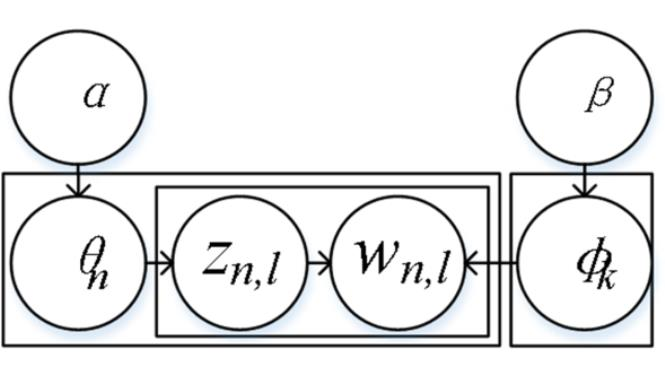
\includegraphics[width=9cm,height=5cm]{res/LDA.jpg}
    \caption{LDA模型图解}
\end{figure} 

如上图所示,LDA 模型假设每个文档都是多个主题的概率分布,每个主题都是多个分词的概率分布,因此文档-分词概率矩阵可以分解为文档-主题概率矩阵与主题-分词概率矩阵。

笔者也为各位读者提供下表以简明介绍上图中符号的意义,并提前说明下文将会使用到的一些符号的意义:

\begin{table}[htbp]
    \centering
    \begin{tabular}{@{}cc@{}}
    \toprule
    符号            & 意义                        \\ \midrule
    $K$           & 主题总数                      \\
    $k$           & 主题编号                      \\
    $Z_{n,l}$     & 文档$n$中第$l$个分词对应的主题编号      \\
    $\alpha$      & 控制文档-主题分布的超参数(狄利克雷分布先验参数) \\
    $\beta$       & 控制主题-词语分布的超参数(狄利克雷分布先验参数) \\
    $w_{n,l}$     & 是文档$n$中第$l$个分词对应的主题编号     \\
    $\theta _{n}$ & 文档$n$的主题分布                \\
    $\varphi_{k}$ & 主题$k$的词汇分布                \\ \bottomrule
    \end{tabular}
\end{table}

接下来,本文将介绍LDA模型的应用过程,该过程也将参考罗文劼与肖梓良老师编写的《融合知识点与图卷积的在线编程题目推荐算法》\cite{LuoRongHeZhiShiDianYuTuJuanJiDeZaiXianBianChengTiMuTuiJianSuanFa}中对LDA模型应用的过程介绍。

首先,在得到给定题目与分词结果的前提下,可以得到$n$与$w_{n,l}$的值。先验参数$\alpha$与$\beta$则采取经验法则,默认设置为$\frac{1}{K}$ 。当然,还有如网格搜索、贝叶斯优化等其他方式选定更优的先验参数,但本文为研究便利,采用较为简单的方式确定先验参数,不采用其他的方式。读者可以根据自身需要尝试选用其他方式确定先验参数。接下来,则使用吉布斯采样法学习LDA模型中的主题分布$\theta _{n}$,过程如下:

\begin{enumerate}
    \item 给定主题总数$K$。
    \item 给每篇文档的每个词汇随机分配主题编号,初始化$Z_{n,l}$。
    \item 利用吉布斯公式对每个词汇进行采样,求出它对应的主题编号,并更新其主题编号$Z_{n,l}$。
    \item 重复上一步骤,直到吉布斯采样收敛或达到迭代次数。
    \item 输出每篇文档的主题分布$\theta _{n}$。
\end{enumerate}

\subsection{基于模糊数学的难度度量模型}

\subsection{}

% ============================================================
%
% 模型的评价与改进
%
% ============================================================

\section{模型的评价与改进}

\subsection{模型的优点}

\begin{itemize}
    \item 12
\end{itemize}

\subsection{模型的缺点}

\subsection{模型的改进}